\section{Desarrollo}


\subsection{Caracterización del STB}
La primera parte consiste en representar las tres salidas del STB y comprobar que se trata de señales senoidales de igual amplitud y frecuencia, separadas aproximadamente \SI{120}{\degree}. En Falstad deben colocarse tres fuentes senoidales con la misma amplitud y frecuencia, modificando la fase de cada una.

\begin{figure}[H]
	\centering
	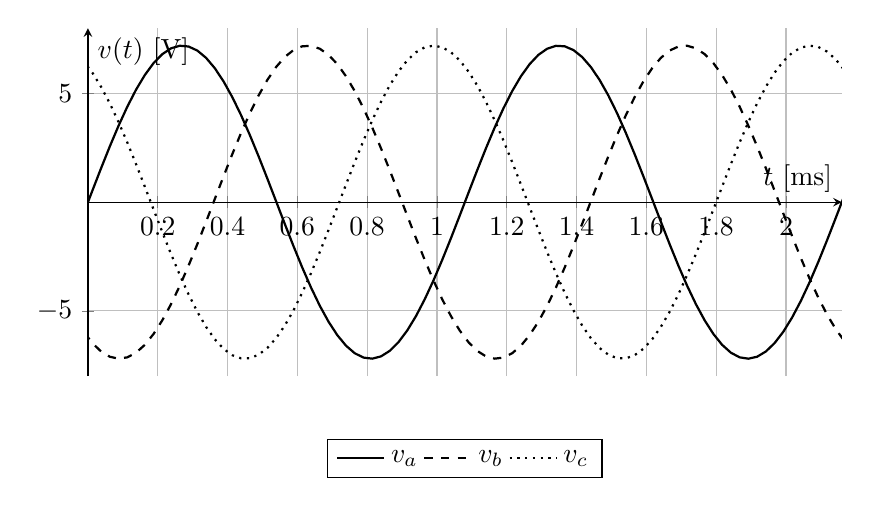
\begin{tikzpicture}
		\begin{axis}[
			width=0.92\textwidth,
			height=6cm,
			axis lines=middle,
			xlabel={$t$ [ms]},
			ylabel={$v(t)$ [V]},
			xmin=0,xmax=2.16,
			ymin=-8,ymax=8,
			samples=400,
			grid=both,
			legend style={at={(0.5,-0.18)},anchor=north,legend columns=3}
			]
			\addplot[thick] {7.2*sin(deg(2*pi*925.93*x/1000))};
			\addlegendentry{$v_a$}
			\addplot[thick,dashed] {7.2*sin(deg(2*pi*925.93*x/1000 - 2*pi/3))};
			\addlegendentry{$v_b$}
			\addplot[thick,dotted] {7.2*sin(deg(2*pi*925.93*x/1000 + 2*pi/3))};
			\addlegendentry{$v_c$}
		\end{axis}
	\end{tikzpicture}
	\caption{Representación teórica de las tres señales generadas por el STB.}
\end{figure}

\begin{figure}[h]
	\centering
	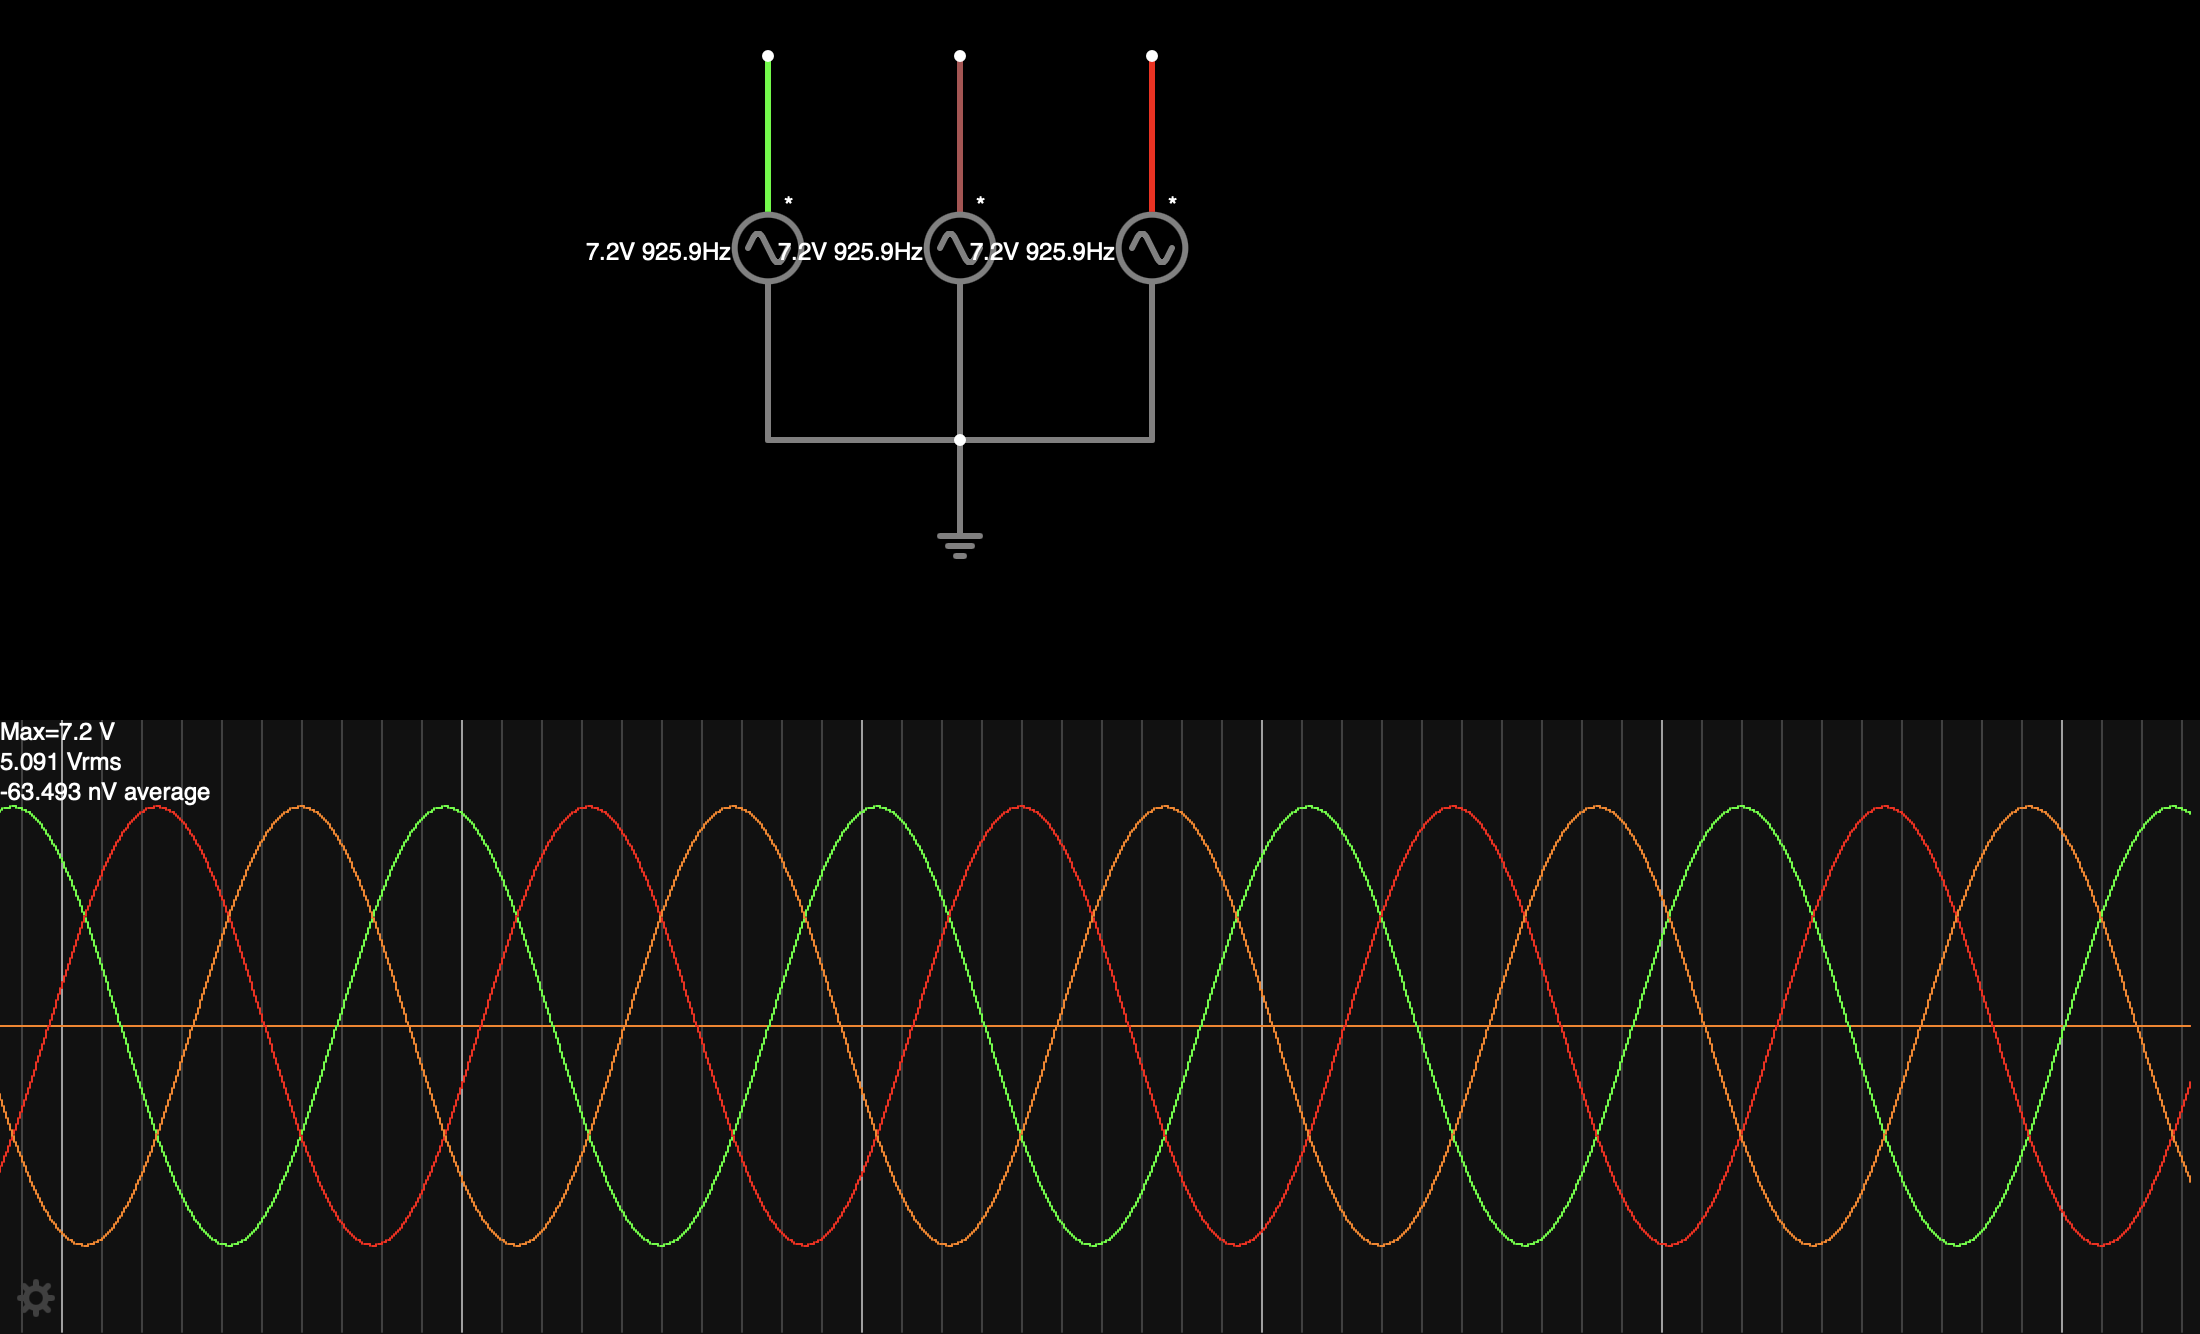
\includegraphics[width=0.9\textwidth]{assets/img/falstad_stb_fases.png}
	\caption{Captura de Falstad del STB con tres fuentes senoidales y osciloscopio mostrando $v_a$, $v_b$ y $v_c$.}
	\label{fig:stb}
\end{figure}

\begin{table}[H]
	\centering
	\caption{Valores teóricos de referencia para la caracterización del STB.}
	\begin{tabular}{lccc}
		\toprule
		Magnitud & Fase $a$ & Fase $b$ & Fase $c$ \\
		\midrule
		Voltaje RMS de fase & \SI{5.091}{V} & \SI{5.091}{V} & \SI{5.091}{V} \\
		Ángulo de fase & $0^{\circ}$ & $-120^{\circ}$ & $120^{\circ}$ \\
		Periodo & \multicolumn{3}{c}{\SI{1.080}{ms}} \\
		Desfase temporal & \multicolumn{3}{c}{\SI{0.360}{ms} entre fases consecutivas} \\
		\bottomrule
	\end{tabular}
\end{table}

\subsection{Voltajes de fase y voltajes de línea}
Al medir entre cada fase y el neutro se obtienen los voltajes de fase. Al medir entre dos fases se obtienen los voltajes de línea. La relación esperada para un sistema balanceado es $V_L/V_F=\sqrt{3}$.

\begin{table}[H]
	\centering
	\caption{Comparación teórica entre voltajes de fase y de línea.}
	\begin{tabular}{lccc}
		\toprule
		Medición & Valor teórico [V RMS] & Relación esperada & Valor en Falstad [V RMS] \\
		\midrule
		$V_{an}$ & 5.091 & -- & 5.091 \\
		$V_{bn}$ & 5.091 & -- & 5.091 \\
		$V_{cn}$ & 5.091 & -- & 5.091 \\
		$V_{ab}$ & 8.818 & $\sqrt{3}V_F$ & 8.818 \\
		$V_{bc}$ & 8.818 & $\sqrt{3}V_F$ & 8.818 \\
		$V_{ca}$ & 8.818 & $\sqrt{3}V_F$ & 8.818 \\
		\bottomrule
	\end{tabular}
\end{table}

\begin{figure}[h]
	\centering
	\begin{subfigure}[b]{0.3\textwidth}
		\centering
		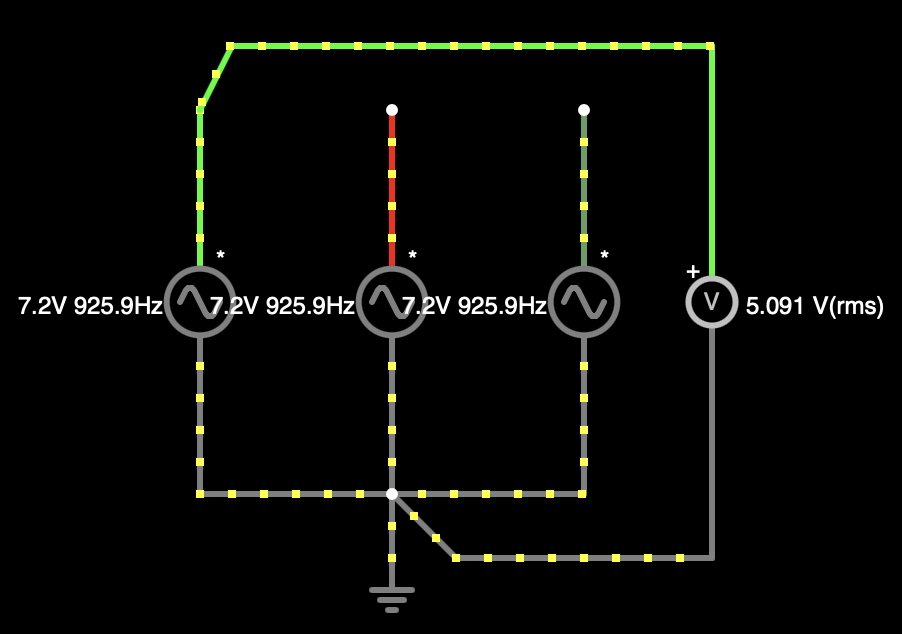
\includegraphics[width=\textwidth]{assets/img/v_an.png}
		\caption{$V_{an}$}
	\end{subfigure}
	\hfill
	\begin{subfigure}[b]{0.3\textwidth}
		\centering
		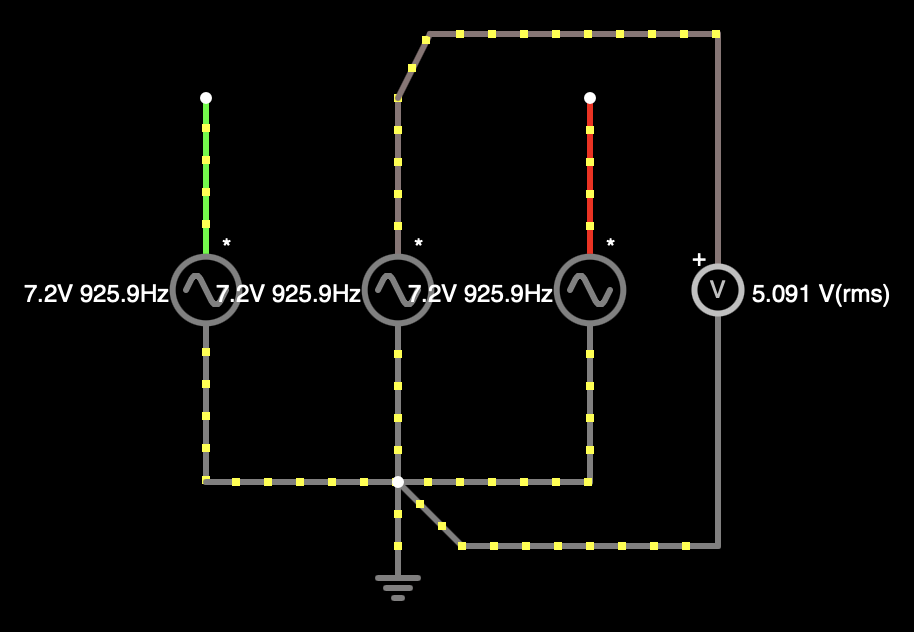
\includegraphics[width=\textwidth]{assets/img/v_bn.png}
		\caption{$V_{bn}$}
	\end{subfigure}
	\hfill
	\begin{subfigure}[b]{0.3\textwidth}
		\centering
		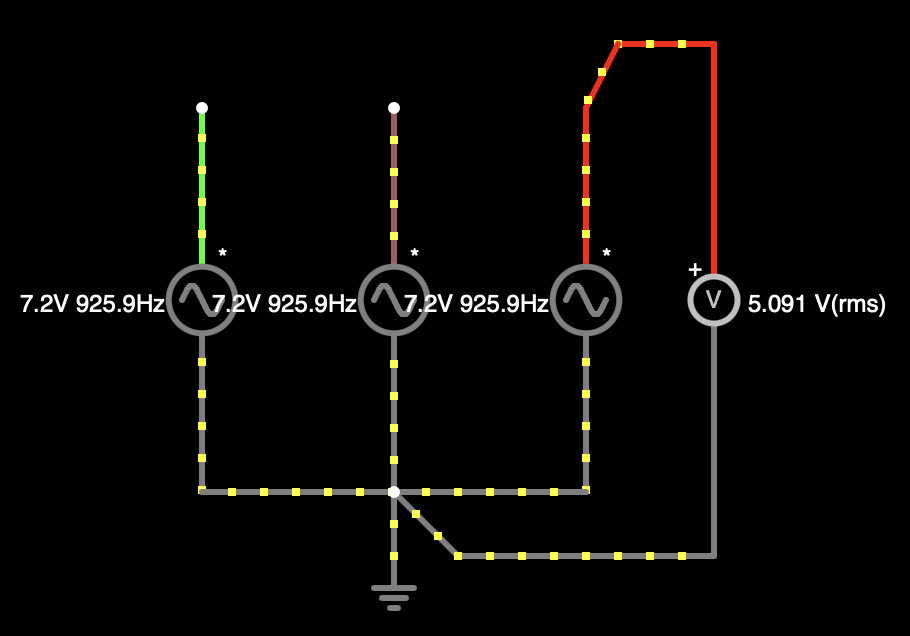
\includegraphics[width=\textwidth]{assets/img/v_cn.png}
		\caption{$V_{cn}$}
	\end{subfigure}
	\caption{Captura de Falstad midiendo $V_{an}$, $V_{bn}$ y $V_{cn}$ con respecto al neutro.}
	\label{fig:stb_linea}
\end{figure}

\begin{figure}[h]
	\centering
	\begin{subfigure}[b]{0.3\textwidth}
		\centering
		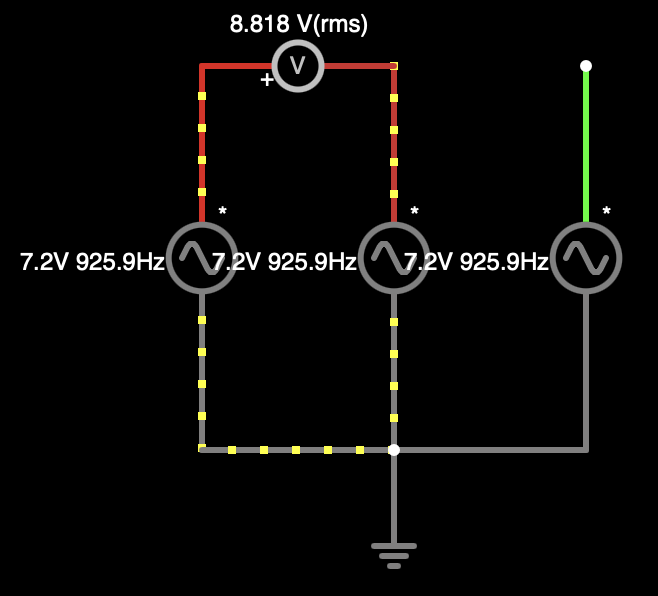
\includegraphics[width=\textwidth]{assets/img/v_ab.png}
		\caption{$V_{ab}$}
	\end{subfigure}
	\hfill
	\begin{subfigure}[b]{0.3\textwidth}
		\centering
		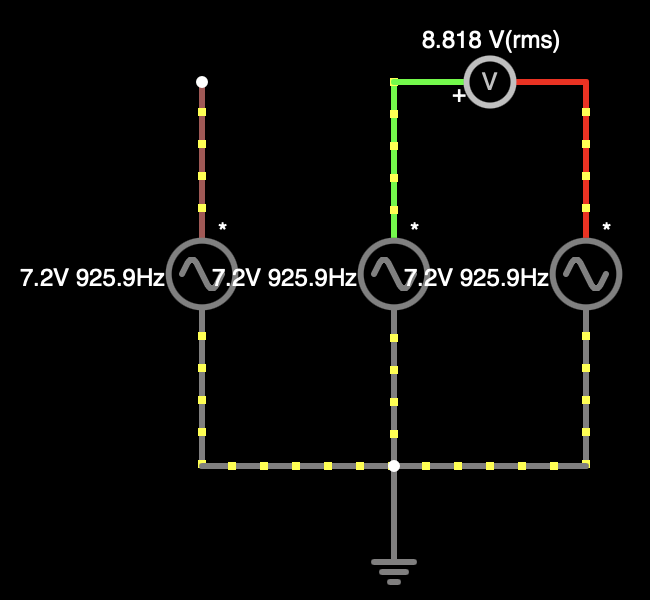
\includegraphics[width=\textwidth]{assets/img/v_bc.png}
		\caption{$V_{bc}$}
	\end{subfigure}
	\hfill
	\begin{subfigure}[b]{0.3\textwidth}
		\centering
		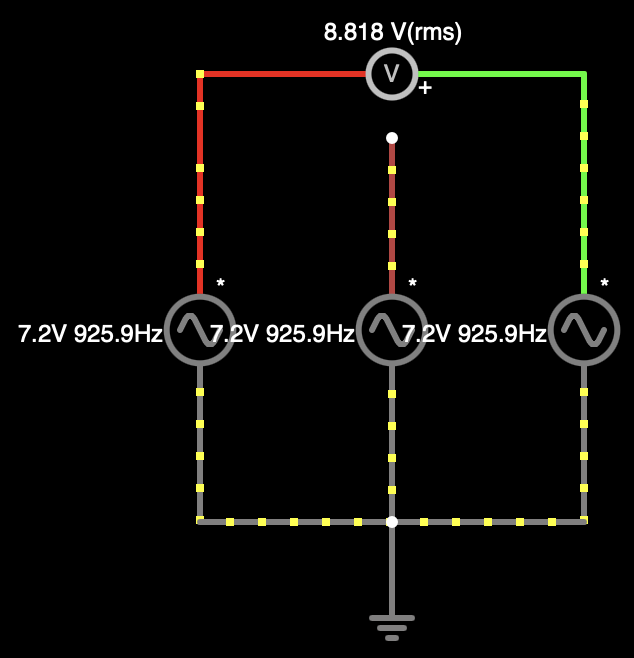
\includegraphics[width=\textwidth]{assets/img/v_ca.png}
		\caption{$V_{ca}$}
	\end{subfigure}
	\caption{Captura de Falstad midiendo $V_{ab}$, $V_{bc}$ y $V_{ca}$ entre líneas.}
	\label{fig:stb_fase}
\end{figure}

\subsection{Carga balanceada en estrella}
Se conectan tres resistencias iguales de \SI{1}{\kilo\ohm} en estrella. Como las tres cargas son iguales, el sistema permanece balanceado.

\begin{figure}[H]
	\centering
	\begin{circuitikz}[scale=1.5]
		\draw (3,3) node[left]{$a$} to[R,l={$R_A=1\,\mathrm{k}\Omega$}] (3,1.5);
		\draw (1,1.5) node[left]{$b$} to[R,l={$R_B=1\,\mathrm{k}\Omega$}] (3,1.5);
		\draw (3,0) node[left]{$c$} to[R,l={$R_C=1\,\mathrm{k}\Omega$}] (3,1.5);
		\draw (3,1.5) -- (4.4,1.5) node[right]{$n'$};
		\draw (4.4,1.5) to[R,l={$r_N=33\,\Omega$}] (4.4,-0.2) node[ground]{};
		\node at (1,2.8) {Carga en estrella};
	\end{circuitikz}
	\caption{Modelo de carga resistiva balanceada en conexión estrella.}
\end{figure}

La corriente en cada fase es:
\begin{equation}
	I_F=\frac{V_F}{R}=\frac{5.091}{1000}=\SI{5.091}{mA}.
\end{equation}

En forma fasorial:
\begin{align}
	\mathbf{I}_a&=\SI{5.091}{mA}\angle 0^{\circ}, \\
	\mathbf{I}_b&=\SI{5.091}{mA}\angle -120^{\circ}, \\
	\mathbf{I}_c&=\SI{5.091}{mA}\angle 120^{\circ}.
\end{align}

Por simetría:
\begin{equation}
	\mathbf{I}_N=\mathbf{I}_a+\mathbf{I}_b+\mathbf{I}_c\approx 0.
\end{equation}

\begin{table}[H]
	\centering
	\caption{Carga estrella balanceada con tres resistencias de \SI{1}{\kilo\ohm}.}
	\begin{tabular}{lccc}
		\toprule
		Rama & Resistencia & Voltaje teórico [V RMS] & Corriente teórica [mA RMS] \\
		\midrule
		$a-n'$ & \SI{1}{\kilo\ohm} & 5.091 & 5.091 \\
		$b-n'$ & \SI{1}{\kilo\ohm} & 5.091 & 5.091 \\
		$c-n'$ & \SI{1}{\kilo\ohm} & 5.091 & 5.091 \\
		Neutro & \SI{33}{\ohm} & $\approx 0$ & $\approx 0$ \\
		\bottomrule
	\end{tabular}
\end{table}

\begin{figure}[h]
	\centering
	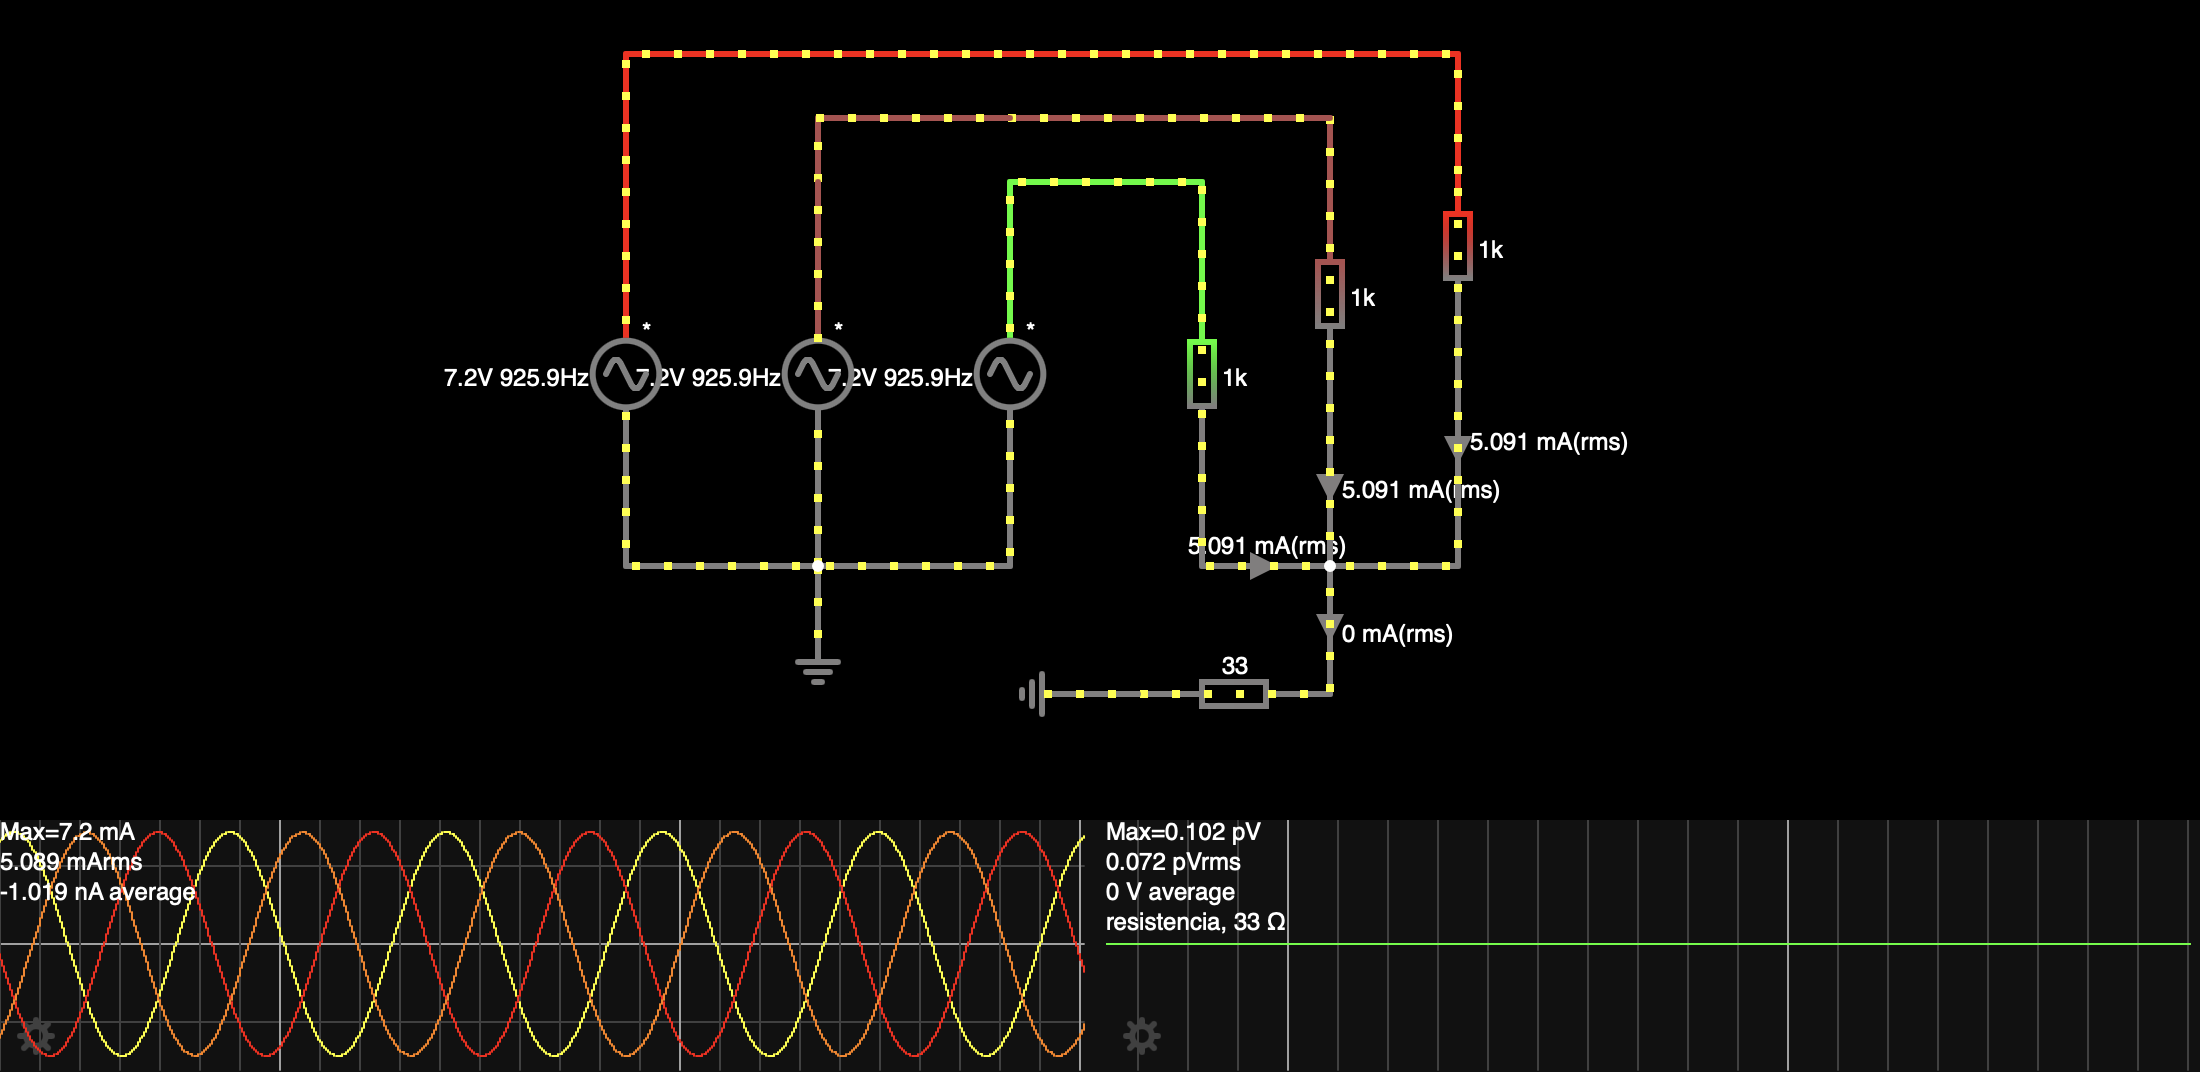
\includegraphics[width=0.9\textwidth]{assets/img/falstad_estrella_balanceada.png}
	\caption{Captura de Falstad de la conexión estrella balanceada, mostrando las corrientes de las tres fases.}
	\label{fig:estrella_balanceada}
\end{figure}

\subsection{Desbalance por pérdida de fase}
Para observar el desbalance por pérdida de fase se desconecta una de las ramas de la estrella. Si se pierde la fase $c$, entonces $I_c=0$ y la corriente de neutro deja de anularse.

Considerando únicamente las ramas $a$ y $b$ conectadas:
\begin{align}
	\mathbf{I}_a&=\SI{5.091}{mA}\angle 0^{\circ}, \\
	\mathbf{I}_b&=\SI{5.091}{mA}\angle -120^{\circ}, \\
	\mathbf{I}_c&=0.
\end{align}

La suma fasorial de $\mathbf{I}_a$ y $\mathbf{I}_b$ produce una corriente de neutro de magnitud aproximada:
\begin{equation}
	|\mathbf{I}_N|\approx\SI{5.091}{mA}.
\end{equation}

Si se emplea una resistencia de medición de \SI{33}{\ohm} en el neutro:
\begin{equation}
	V_{r_N}=I_Nr_N=(5.091\times10^{-3})(33)=\SI{0.168}{V_{RMS}}.
\end{equation}

\begin{figure}[h]
	\centering
	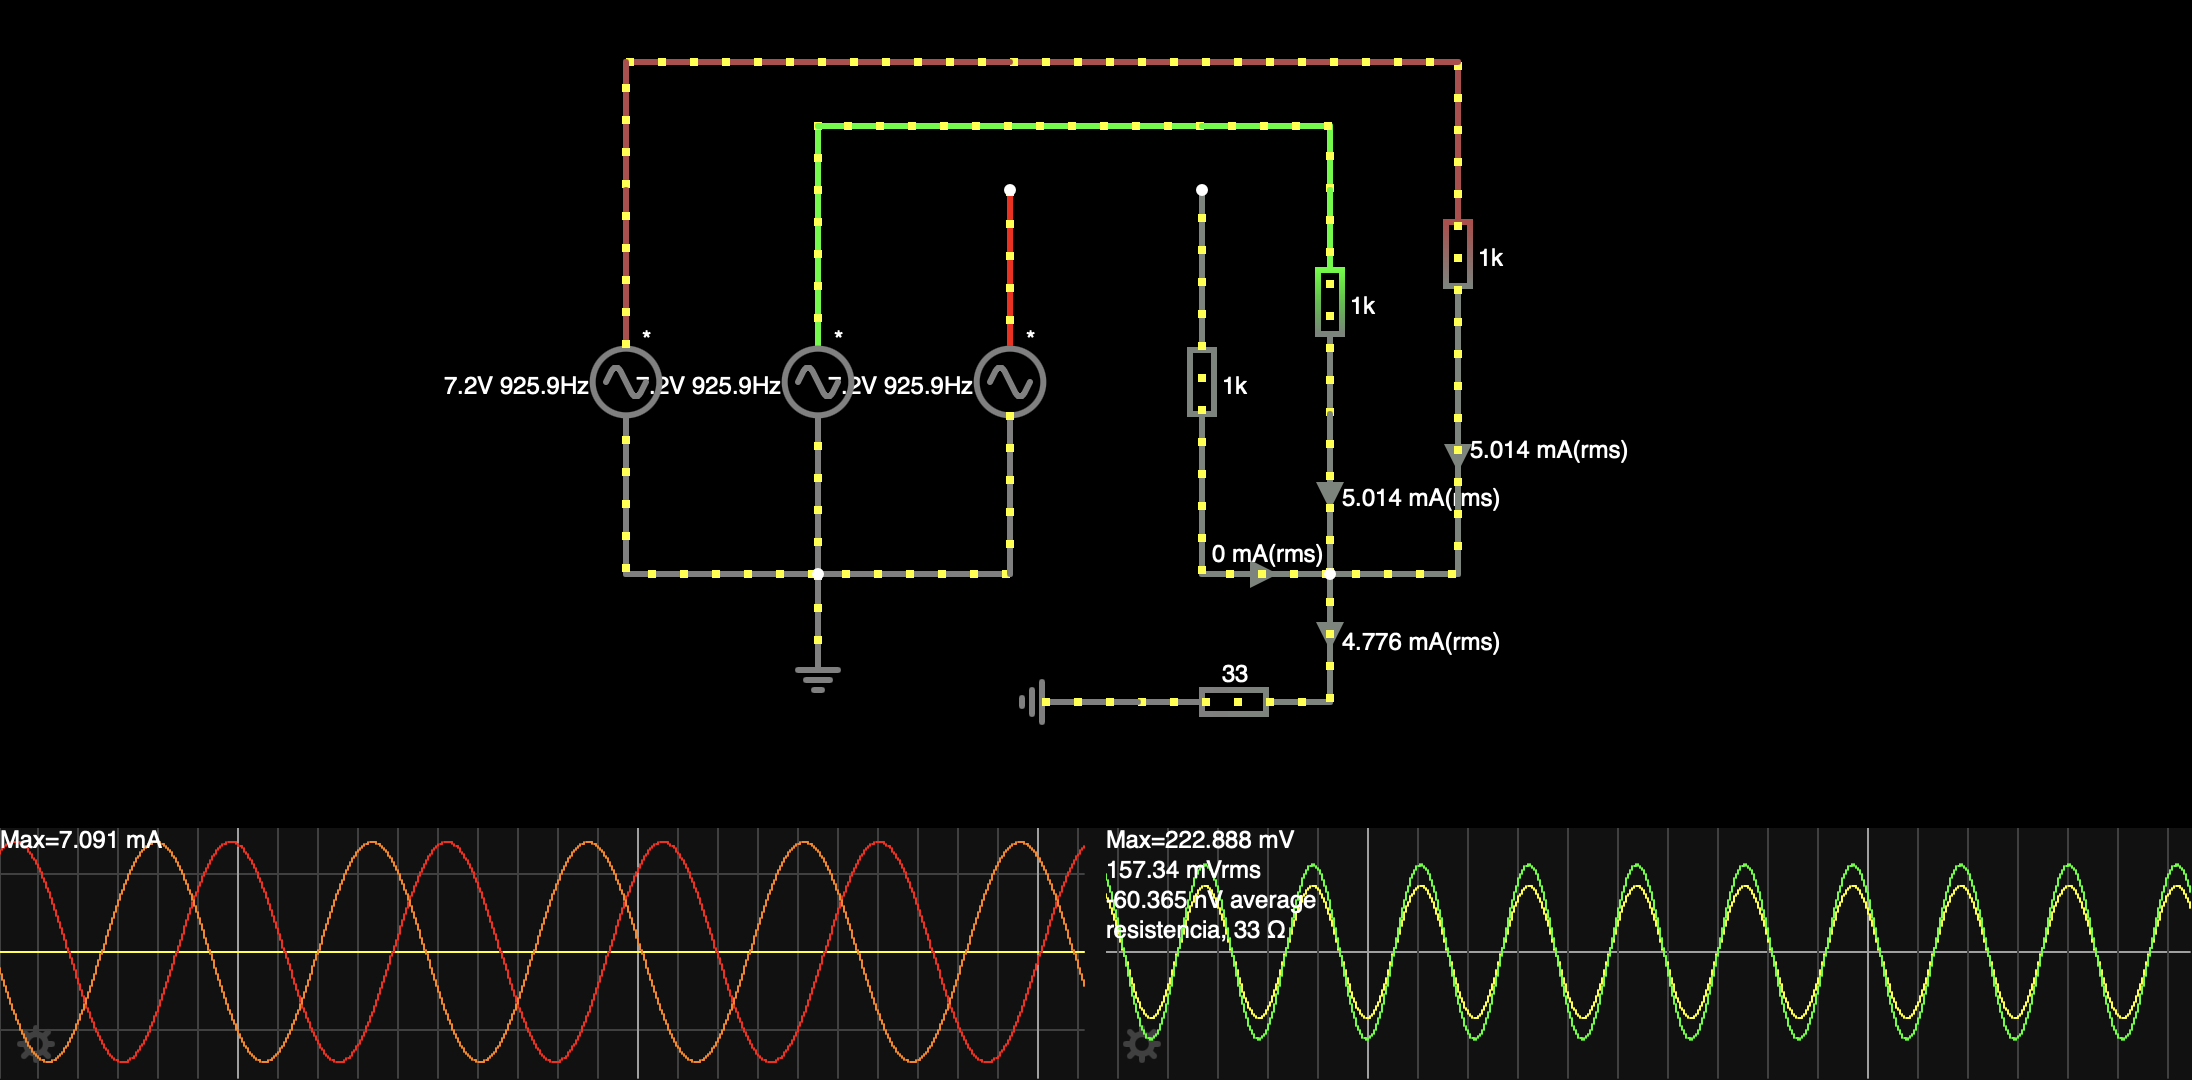
\includegraphics[width=0.9\textwidth]{assets/img/falstad_perdida_fase.png}
	\caption{Captura de Falstad de la estrella con pérdida de una fase y medición de corriente/voltaje en el neutro.}
	\label{fig:estrella_perdida_fase}
\end{figure}

\subsection{Desbalance por impedancias distintas}
En este caso se conservan las tres fases conectadas, pero una carga se cambia por una resistencia de valor diferente. Como ejemplo teórico se considera:
\begin{equation}
	R_A=\SI{1}{\kilo\ohm},\quad R_B=\SI{1}{\kilo\ohm},\quad R_C=\SI{22}{\kilo\ohm}.
\end{equation}

Las corrientes resultantes son:
\begin{align}
	|\mathbf{I}_a|&=\frac{5.091}{1000}=\SI{5.091}{mA}, \\
	|\mathbf{I}_b|&=\frac{5.091}{1000}=\SI{5.091}{mA}, \\
	|\mathbf{I}_c|&=\frac{5.091}{22000}=\SI{0.231}{mA}.
\end{align}

La suma fasorial no se cancela, por lo que se obtiene:
\begin{equation}
	|\mathbf{I}_N|\approx\SI{4.860}{mA},\quad \angle \mathbf{I}_N\approx -60^{\circ}.
\end{equation}

\begin{table}[H]
	\centering
	\caption{Ejemplo de estrella desbalanceada por resistencia distinta.}
	\begin{tabular}{lccc}
		\toprule
		Rama & Impedancia & Corriente teórica [mA RMS] & Valor en Falstad [mA RMS] \\
		\midrule
		$a-n'$ & \SI{1}{\kilo\ohm} & 5.091 & 5.018 \\
		$b-n'$ & \SI{1}{\kilo\ohm} & 5.091 & 5.018 \\
		$c-n'$ & \SI{22}{\kilo\ohm} & 0.231 & 0.238 \\
		Neutro & -- & 4.860 & 4.552 \\
		\bottomrule
	\end{tabular}
\end{table}

\begin{figure}[h]
	\centering
	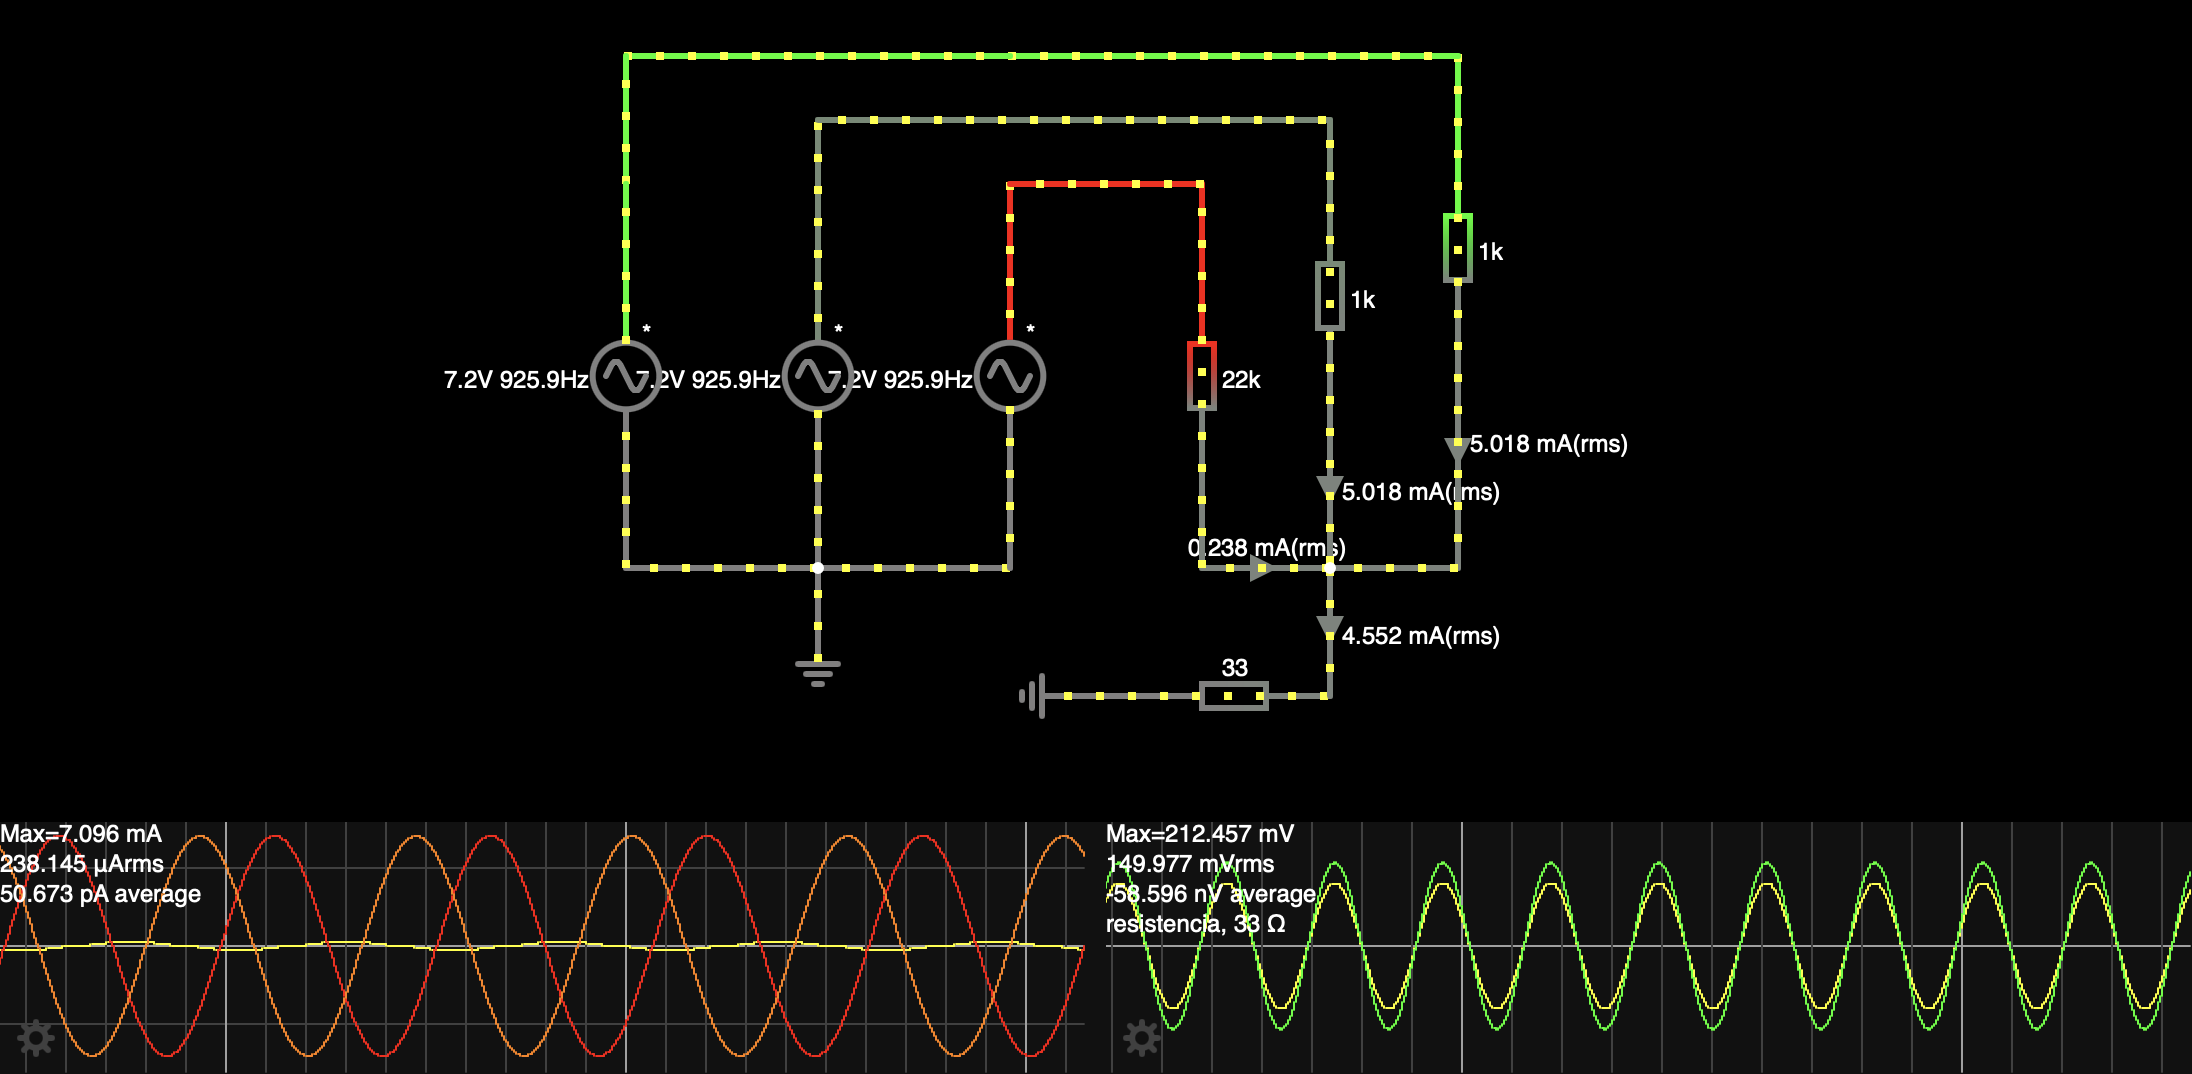
\includegraphics[width=0.9\textwidth]{assets/img/falstad_estrella_desbalance_resistiva.png}
	\caption{Captura de Falstad de estrella con dos resistencias de \SI{1}{\kilo\ohm} y una de \SI{22}{\kilo\ohm}.}
	\label{fig:estrella_desbalance_resistiva}
\end{figure}

\subsection{Neutro flotante con carga desbalanceada}
Cuando el neutro se desconecta, el nodo común $n'$ ya no se mantiene al potencial del neutro de la fuente. Si las cargas no son iguales, el punto $n'$ se desplaza y los voltajes de fase en las cargas dejan de ser iguales.

Para mostrar este efecto se propone una simulación con:
\begin{equation}
	Z_A=\SI{1}{\kilo\ohm},\quad Z_B=\SI{22}{\kilo\ohm},\quad Z_C=-j\SI{781.30}{\ohm}.
\end{equation}

El voltaje del neutro flotante se calcula mediante análisis nodal:
\begin{equation}
	\mathbf{V}_{n'}=\frac{Y_A\mathbf{V}_a+Y_B\mathbf{V}_b+Y_C\mathbf{V}_c}{Y_A+Y_B+Y_C},
\end{equation}

con $Y_k=1/Z_k$. Para los valores anteriores:
\begin{equation}
	|\mathbf{V}_{n'}|\approx\SI{2.131}{V_{RMS}},\quad \angle \mathbf{V}_{n'}\approx -151.69^{\circ}.
\end{equation}

Los voltajes de carga resultan:
\begin{table}[H]
	\centering
	\caption{Voltajes teóricos en cargas con neutro flotante.}
	\begin{tabular}{lccc}
		\toprule
		Rama & Impedancia & Voltaje teórico [V RMS] & Corriente teórica [mA RMS] \\
		\midrule
		$a-n'$ & \SI{1}{\kilo\ohm} & 7.041 & 7.041 \\
		$b-n'$ & \SI{22}{\kilo\ohm} & 3.463 & 0.157 \\
		$c-n'$ & $-j\SI{781.30}{\ohm}$ & 5.461 & 6.990 \\
		$n'-n$ & -- & 2.131 & -- \\
		\bottomrule
	\end{tabular}
\end{table}

\begin{figure}[h]
	\centering
	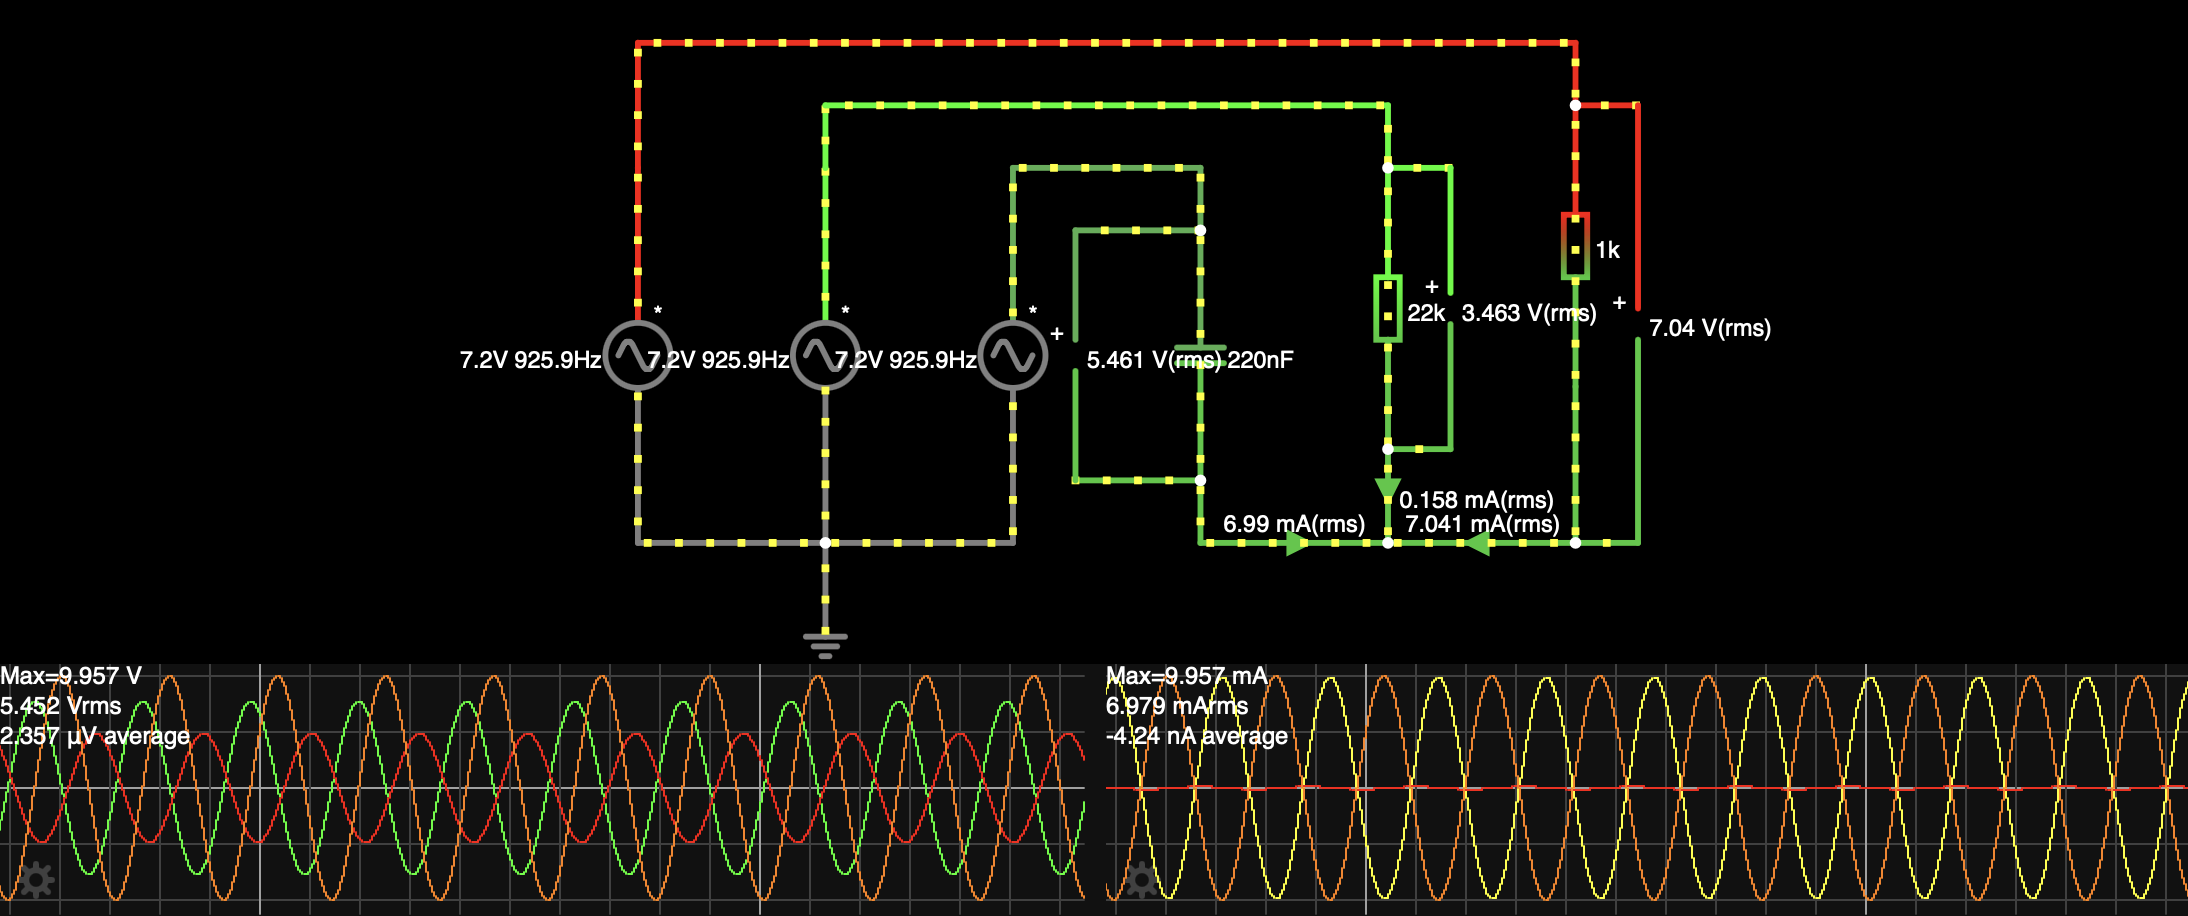
\includegraphics[width=0.9\textwidth]{assets/img/falstad_neutro_flotante.png}
	\caption{Captura de Falstad de la carga desbalanceada con neutro abierto o flotante.}
	\label{fig:neutro_flotante}
\end{figure}

\subsection{Carga balanceada en delta}
En conexión delta se colocan tres resistencias iguales entre pares de líneas. Para una delta resistiva con $R=\SI{1}{\kilo\ohm}$, cada resistencia queda sometida al voltaje de línea $V_L=\SI{8.818}{V_{RMS}}$.

\begin{figure}[H]
	\centering
	\begin{circuitikz}[scale=1.25]
		\coordinate (A) at (0,3);
		\coordinate (B) at (-2,0);
		\coordinate (C) at (2,0);
		\draw (A) to[R,l={$R_{AB}=1\,\mathrm{k}\Omega$}] (B);
		\draw (B) to[R,l={$R_{BC}=1\,\mathrm{k}\Omega$}] (C);
		\draw (C) to[R,l={$R_{CA}=1\,\mathrm{k}\Omega$}] (A);
		\draw (A) -- (0,4) node[above]{$a$};
		\draw (B) -- (-3,0) node[left]{$b$};
		\draw (C) -- (3,0) node[right]{$c$};
		\node at (0,1) {Delta};
	\end{circuitikz}
	\caption{Conexión delta resistiva balanceada.}
\end{figure}

La corriente de fase en cada resistencia es:
\begin{equation}
	I_F^{(\Delta)}=\frac{V_L}{R}=\frac{8.818}{1000}=\SI{8.818}{mA}.
\end{equation}

La corriente de línea esperada es:
\begin{equation}
	I_L=\sqrt{3}I_F=\sqrt{3}(8.818)=\SI{15.274}{mA}.
\end{equation}

Si se coloca una resistencia de \SI{33}{\ohm} como resistencia de sensado en serie con cada línea, el voltaje esperado en ella es:
\begin{equation}
	V_{33\Omega}=I_L(33)=\SI{0.504}{V_{RMS}}.
\end{equation}

\begin{table}[H]
	\centering
	\caption{Carga delta balanceada con resistencias de \SI{1}{\kilo\ohm}.}
	\begin{tabular}{lccc}
		\toprule
		Elemento & Resistencia & Voltaje [V RMS] & Corriente [mA RMS] \\
		\midrule
		$R_{AB}$ & \SI{1}{\kilo\ohm} & 8.818 & 8.818 \\
		$R_{BC}$ & \SI{1}{\kilo\ohm} & 8.818 & 8.818 \\
		$R_{CA}$ & \SI{1}{\kilo\ohm} & 8.818 & 8.818 \\
		Línea $a$ & \SI{33}{\ohm} como sensor & 0.504 & 15.274 \\
		Línea $b$ & \SI{33}{\ohm} como sensor & 0.504 & 15.274 \\
		Línea $c$ & \SI{33}{\ohm} como sensor & 0.504 & 15.274 \\
		\bottomrule
	\end{tabular}
\end{table}

\begin{figure}[h]
	\centering
	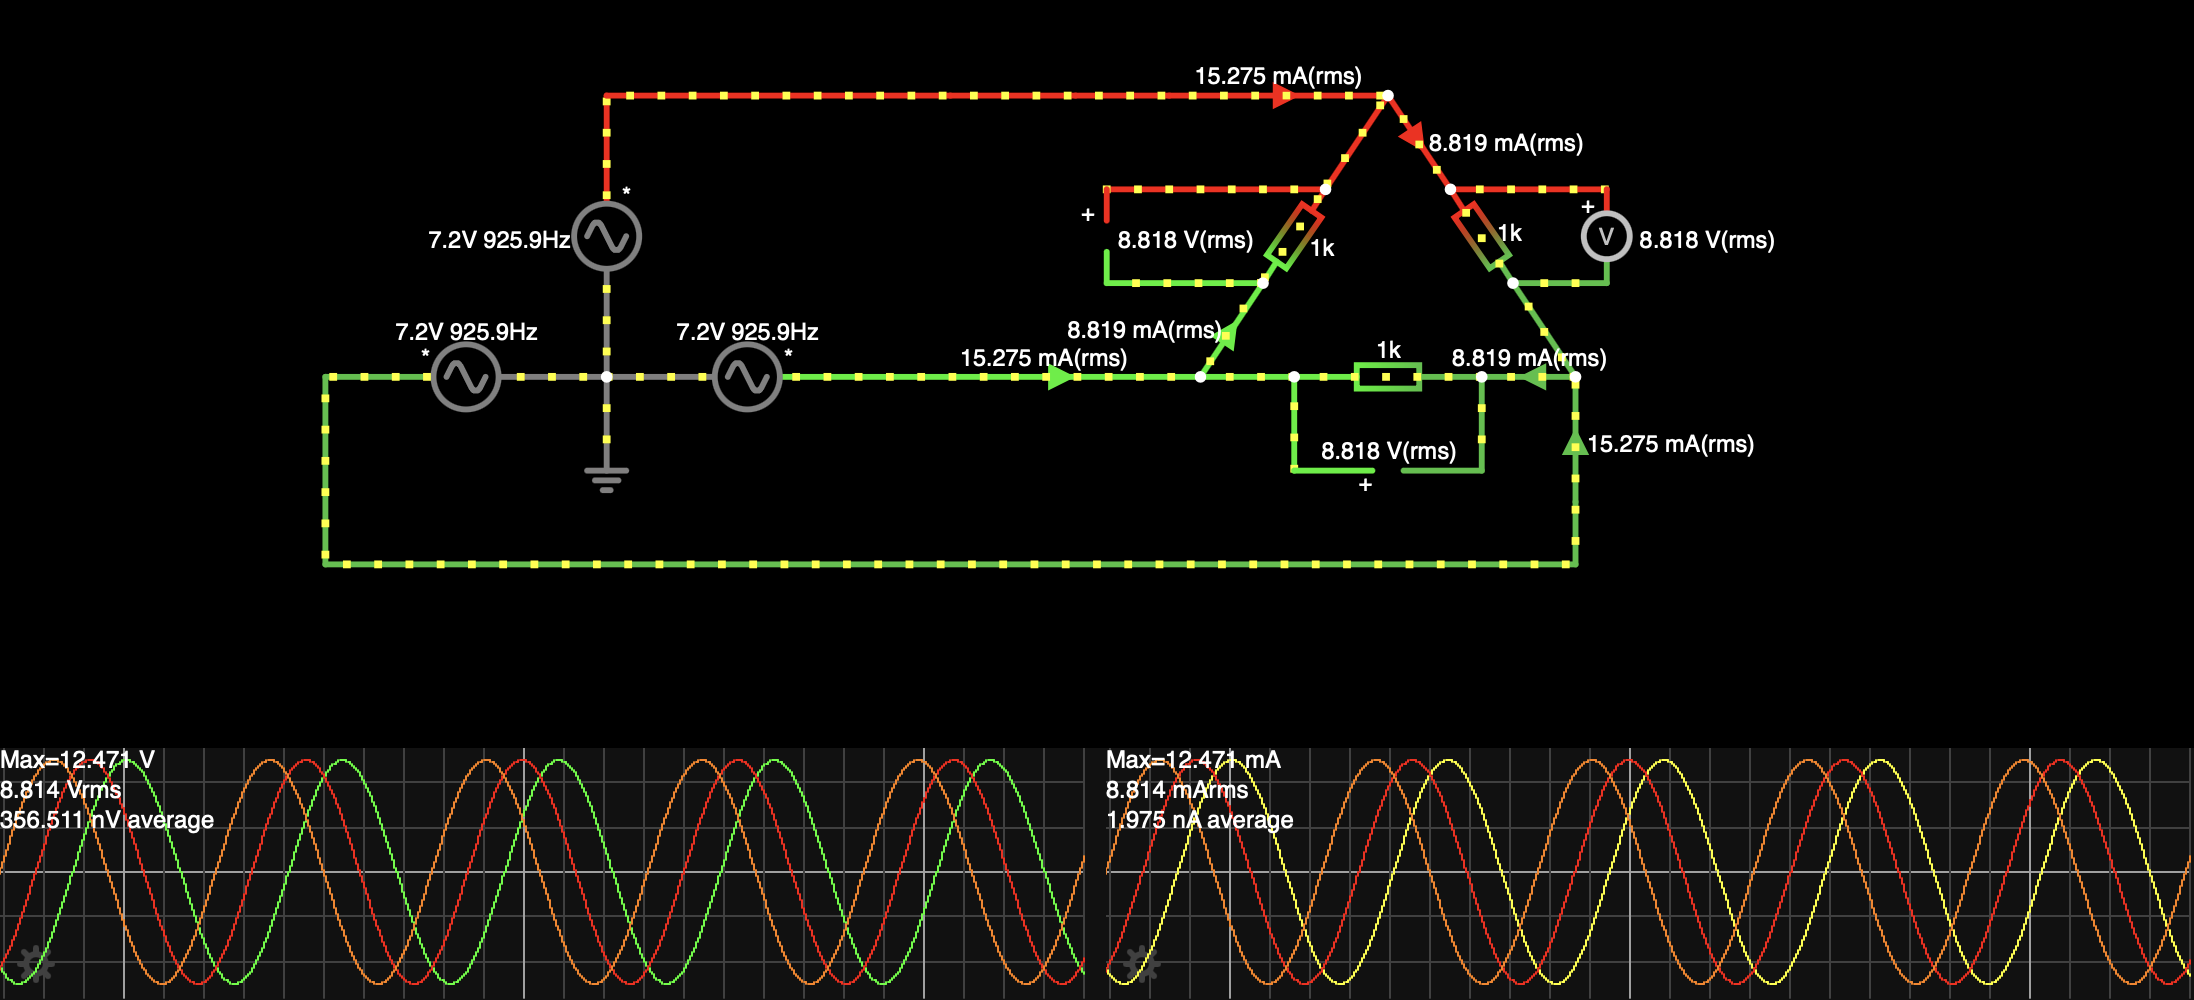
\includegraphics[width=0.9\textwidth]{assets/img/falstad_delta_balanceada.png}
	\caption{Captura de Falstad de la conexión delta balanceada, mostrando corrientes de fase y corrientes de línea.}
	\label{fig:delta_balanceada}
\end{figure}

\subsection{Carga delta desbalanceada}
Para analizar el efecto de una delta desbalanceada se propone sustituir una de las resistencias por \SI{22}{\kilo\ohm}:
\begin{equation}
	R_{AB}=\SI{1}{\kilo\ohm},\quad R_{BC}=\SI{1}{\kilo\ohm},\quad R_{CA}=\SI{22}{\kilo\ohm}.
\end{equation}

Las corrientes de fase son:
\begin{align}
	|I_{AB}|&=\SI{8.818}{mA}, \\
	|I_{BC}|&=\SI{8.818}{mA}, \\
	|I_{CA}|&=\frac{8.818}{22000}=\SI{0.401}{mA}.
\end{align}

La suma vectorial de corrientes en cada nodo produce corrientes de línea diferentes:
\begin{table}[H]
	\centering
	\caption{Corrientes teóricas en una delta desbalanceada.}
	\begin{tabular}{lcc}
		\toprule
		Corriente & Magnitud teórica [mA RMS] & Ángulo aproximado \\
		\midrule
		$I_{AB}$ & 8.818 & $30^{\circ}$ \\
		$I_{BC}$ & 8.818 & $-90^{\circ}$ \\
		$I_{CA}$ & 0.401 & $150^{\circ}$ \\
		$I_a$ & 9.025 & $27.80^{\circ}$ \\
		$I_b$ & 15.274 & $-120^{\circ}$ \\
		$I_c$ & 9.025 & $92.20^{\circ}$ \\
		\bottomrule
	\end{tabular}
\end{table}

\begin{figure}[h]
	\centering
	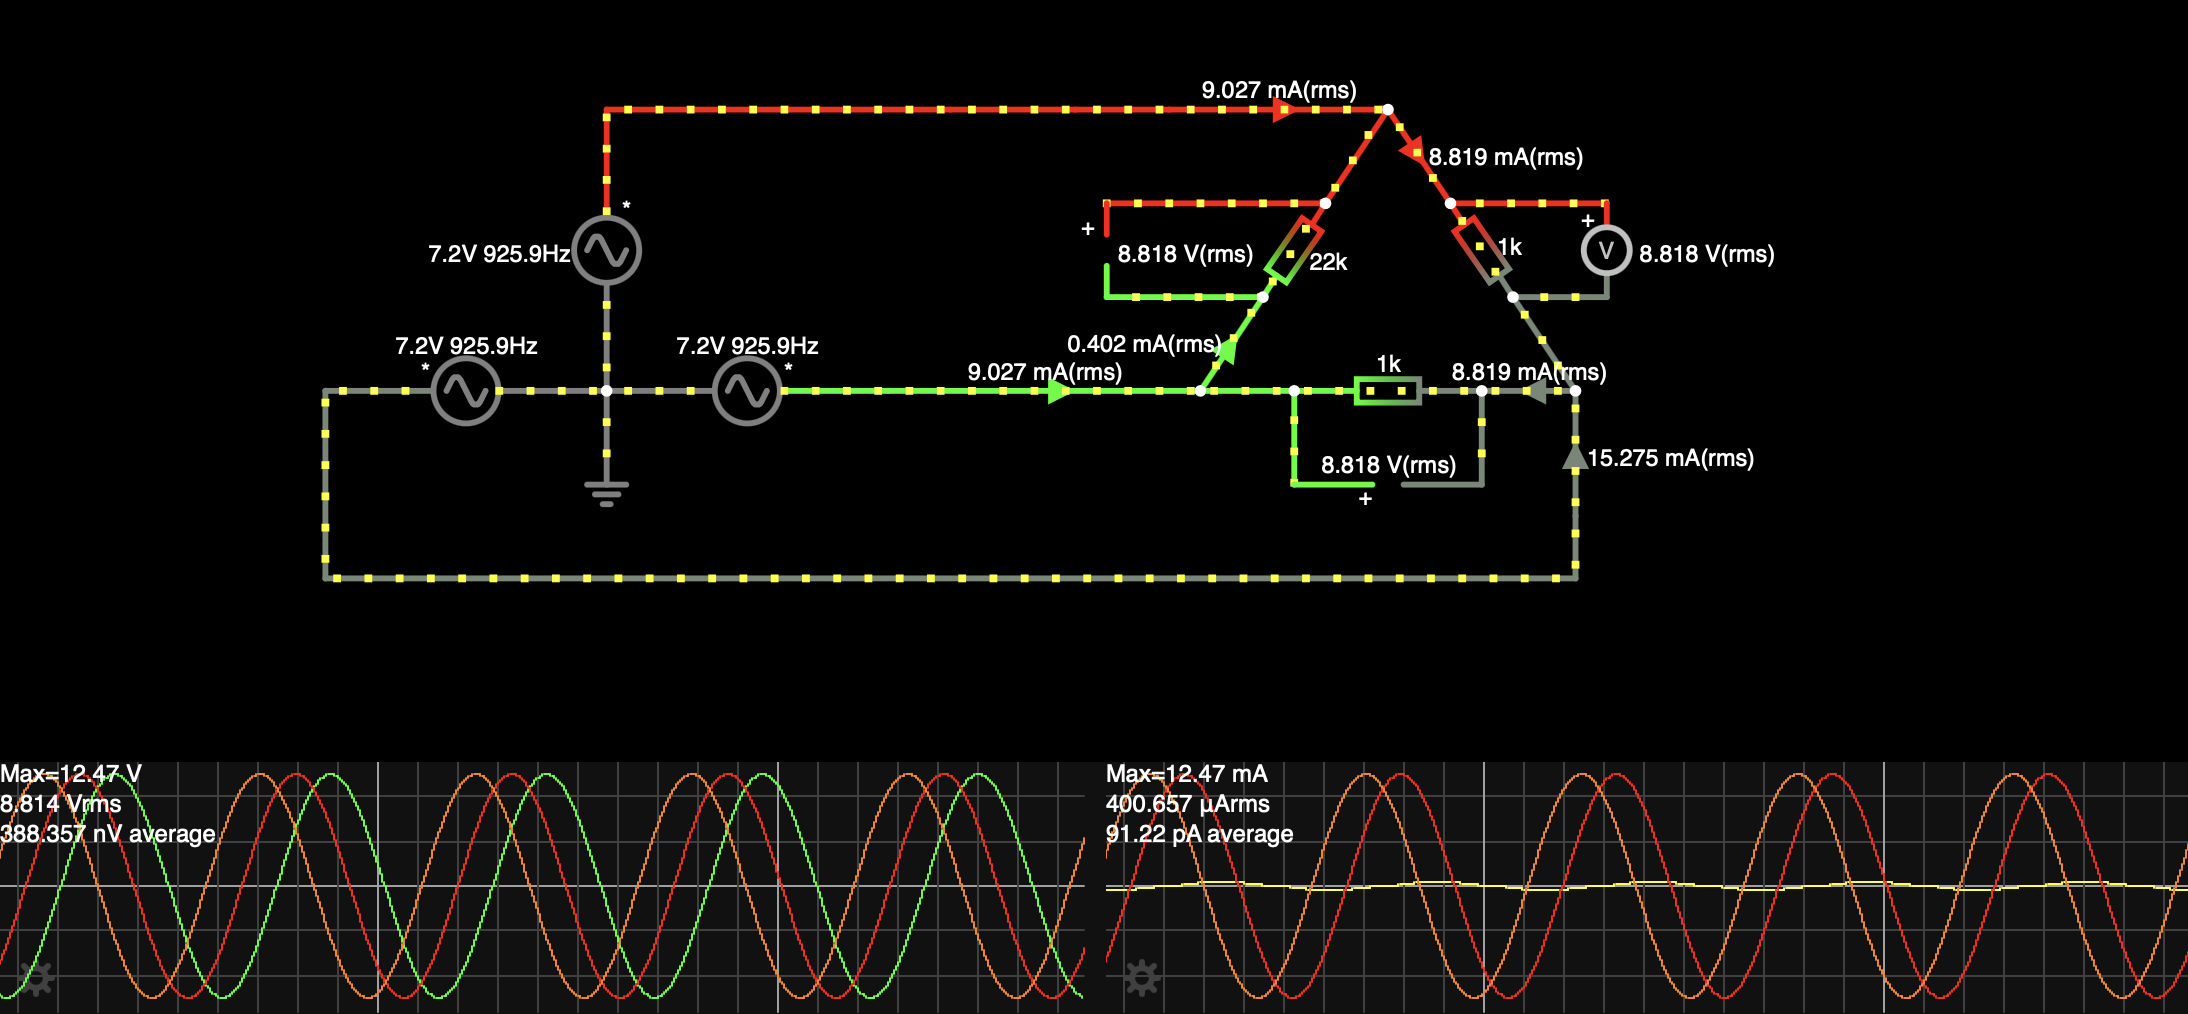
\includegraphics[width=0.9\textwidth]{assets/img/falstad_delta_desbalanceada.png}
	\caption{Captura de Falstad de delta desbalanceada con dos resistencias de \SI{1}{\kilo\ohm} y una de \SI{22}{\kilo\ohm}.}
	\label{fig:delta_desbalanceada}
\end{figure}

\section{Análisis de resultados}

\subsection{Relación entre voltajes de línea y fase}

En el sistema trifásico balanceado, los voltajes de fase tienen la misma magnitud y están separados
angularmente $120^\circ$. Al obtener los voltajes de línea mediante la resta fasorial entre dos voltajes
de fase, se observa que su magnitud aumenta en un factor de $\sqrt{3}$ y que aparece un desplazamiento
angular de $30^\circ$.

Por lo tanto, para el STB utilizado en la práctica se cumple:

\[
V_L = \sqrt{3}V_F
\]

Sustituyendo el valor teórico de fase:

\[
V_L = \sqrt{3}(5.091) = 8.818 \; V_{RMS}
\]

Esto coincide con las mediciones realizadas en Falstad, donde los voltajes entre líneas fueron
aproximadamente $8.818 \; V_{RMS}$.

\begin{figure}[H]
	\centering
	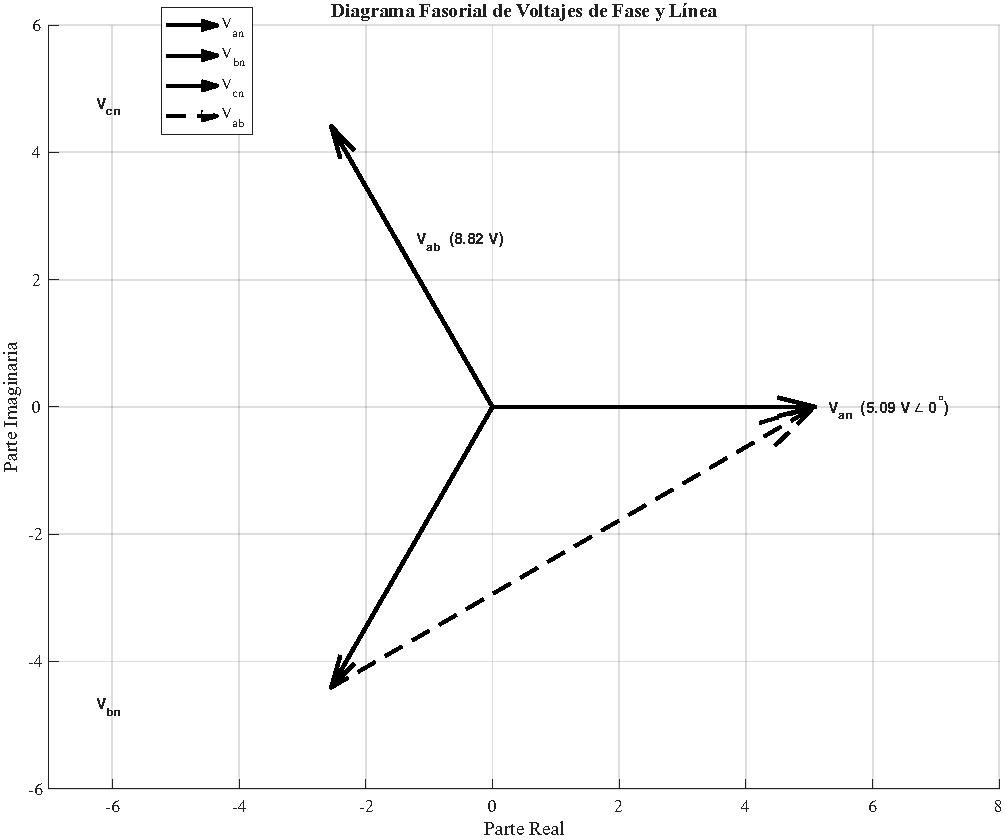
\includegraphics[width=0.70\textwidth]{assets/img/1.pdf}
	\caption{Diagrama fasorial de voltajes de fase y voltaje de línea.}
	\label{fig:fasores_voltajes}
\end{figure}

\subsection{Corriente de neutro en estrella balanceada}

En la conexión estrella balanceada, las tres impedancias son iguales. Por ello, las corrientes de fase
tienen la misma magnitud y mantienen el mismo desfase de $120^\circ$ que los voltajes de alimentación.

Para resistencias de $1\,k\Omega$, la corriente de fase teórica es:

\[
I_F = \frac{V_F}{R} = \frac{5.091}{1000} = 5.091 \; mA
\]

La suma fasorial de las tres corrientes es:

\[
I_N = I_a + I_b + I_c
\]

Como las tres corrientes forman un sistema balanceado, su suma es aproximadamente cero:

\[
I_N \approx 0
\]

Esto explica por qué en la simulación la corriente por el neutro fue prácticamente nula.

\begin{figure}[H]
	\centering
	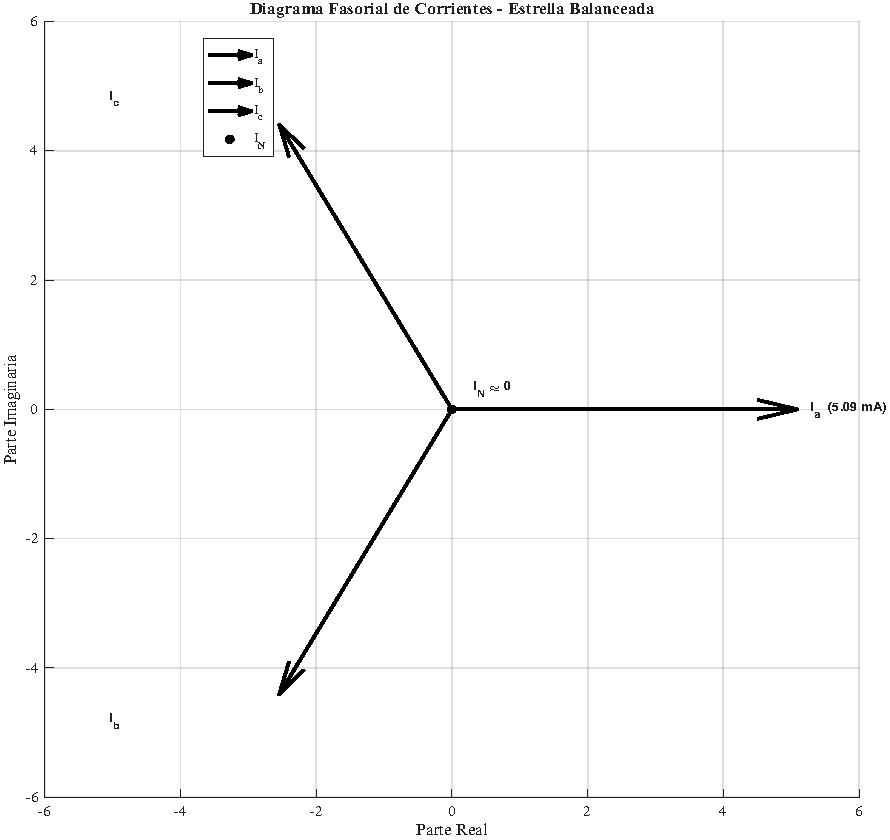
\includegraphics[width=0.70\textwidth]{assets/img/2.pdf}
	\caption{Diagrama fasorial de corrientes en estrella balanceada.}
	\label{fig:fasores_estrella_balanceada}
\end{figure}

\subsection{Corriente de neutro en estrella desbalanceada}

Cuando las impedancias de la carga dejan de ser iguales, las corrientes de fase ya no tienen la misma
magnitud. Aunque continúan asociadas a fases separadas $120^\circ$, la suma fasorial ya no se anula.
Por esta razón aparece una corriente por el neutro.

Para el caso con:

\[
R_A = 1\,k\Omega, \qquad R_B = 1\,k\Omega, \qquad R_C = 22\,k\Omega
\]

las corrientes teóricas son:

\[
I_a = 5.091 \; mA
\]

\[
I_b = 5.091 \; mA
\]

\[
I_c = 0.231 \; mA
\]

Debido a que la corriente de la fase $c$ es mucho menor que las otras dos, el sistema deja de estar
balanceado y aparece una corriente resultante en el neutro:

\[
I_N = I_a + I_b + I_c
\]

La magnitud esperada es aproximadamente:

\[
|I_N| \approx 4.860 \; mA
\]

Este resultado coincide con el comportamiento observado en Falstad, donde la corriente de neutro
aumentó al introducir una carga desbalanceada.

\begin{figure}[H]
	\centering
	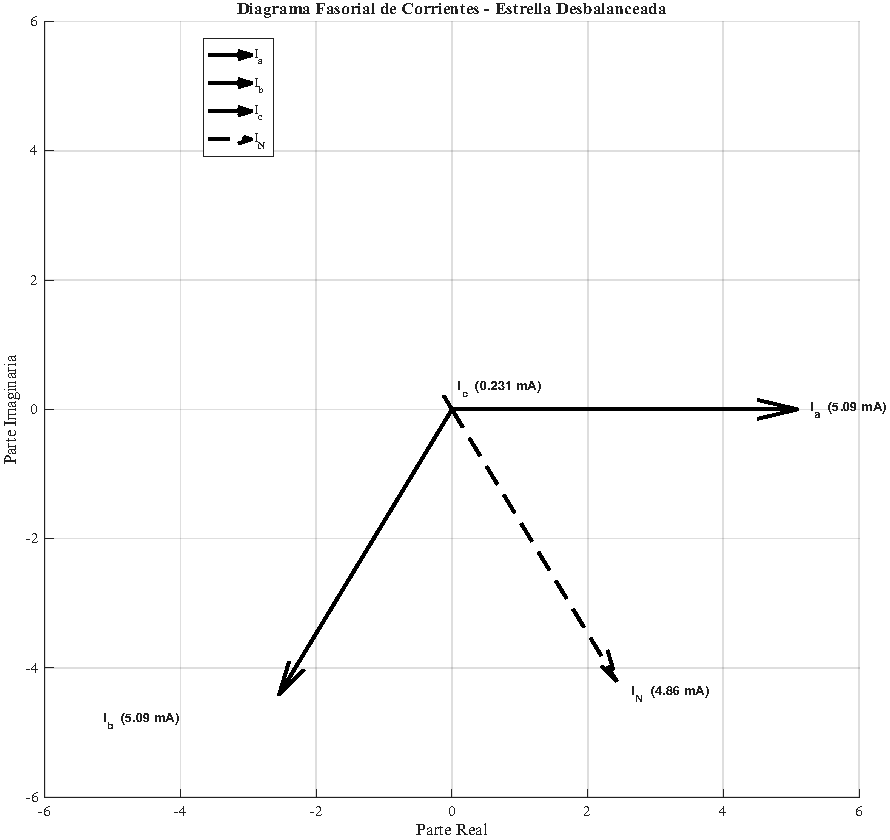
\includegraphics[width=0.70\textwidth]{assets/img/3.pdf}
	\caption{Diagrama fasorial de corrientes en estrella desbalanceada.}
	\label{fig:fasores_estrella_desbalanceada}
\end{figure}

\subsection{Neutro flotante}

En el caso de neutro flotante, el nodo común de la carga $n'$ no está conectado directamente al neutro
de la fuente. Por esta razón, su potencial depende de las admitancias de cada rama. Si la carga es
desbalanceada, el punto $n'$ se desplaza respecto al neutro real del sistema.

Este desplazamiento provoca que los voltajes aplicados a cada carga ya no sean iguales. Para el caso:

\[
Z_A = 1\,k\Omega, \qquad Z_B = 22\,k\Omega, \qquad Z_C = -j781.30\,\Omega
\]

se obtuvo teóricamente:

\[
|V_{n'}| \approx 2.131 \; V_{RMS}
\]

Por ello, en la simulación de Falstad se espera observar que el nodo común de la carga presenta un
voltaje distinto de cero respecto al neutro de la fuente.

\subsection{Relación de corrientes en delta}

En la conexión delta balanceada, cada impedancia queda conectada entre dos líneas. Por lo tanto, el
voltaje aplicado a cada rama de la delta es el voltaje de línea:

\[
V_F^{(\Delta)} = V_L
\]

Para resistencias de $1\,k\Omega$:

\[
I_F^{(\Delta)} = \frac{V_L}{R} = \frac{8.818}{1000} = 8.818 \; mA
\]

Sin embargo, la corriente de línea no es igual a la corriente de fase, ya que cada línea alimenta dos
ramas de la delta. En condición balanceada se cumple:

\[
I_L = \sqrt{3}I_F
\]

Por lo tanto:

\[
I_L = \sqrt{3}(8.818) = 15.274 \; mA
\]

Este resultado permite verificar en Falstad que, aunque la corriente en cada resistencia es de
aproximadamente $8.818 \; mA$, la corriente de línea es mayor debido a la suma fasorial de corrientes
en cada nodo de la delta.

%---------------------------- CONCLUSIONES ----------------------------
\section{Conclusiones}
Con el desarrollo de esta práctica se comprobó la utilidad del análisis fasorial para estudiar circuitos trifásicos en régimen senoidal permanente. Al representar las salidas del STB como tres señales senoidales de igual magnitud y separadas \SI{120}{\degree}, fue posible obtener las relaciones fundamentales entre voltajes de fase, voltajes de línea y corrientes en diferentes configuraciones.

En conexión estrella balanceada, las corrientes de fase son iguales a las corrientes de línea y su suma fasorial en el neutro tiende a cero. Esto permite identificar el comportamiento ideal de un sistema balanceado. Cuando se desconecta una fase o se cambia una impedancia, la suma de corrientes deja de anularse, lo cual se manifiesta como corriente de neutro y como diferencias de voltaje entre ramas.

El análisis del neutro flotante mostró que la desconexión del neutro no siempre produce un problema si las cargas son perfectamente balanceadas; sin embargo, bajo condiciones de desbalance el punto común se desplaza y modifica los voltajes aplicados a cada carga. Este fenómeno es relevante porque puede causar sobretensiones o subtensiones en ramas específicas.

Finalmente, en conexión delta se observó que el voltaje de fase coincide con el voltaje de línea, mientras que la corriente de línea se obtiene como suma fasorial de corrientes de fase. En el caso balanceado se cumple $I_L=\sqrt{3}I_F$; en el caso desbalanceado esta relación deja de cumplirse de forma uniforme, por lo que debe analizarse cada rama de manera individual.
